% !TeX root = thesis_main.tex
% ---------------------------------------------------
% ----- Main document of the template
% ----- for Bachelor-, Master thesis and class papers
% ---------------------------------------------------
%  Created by C. Müller-Birn on 2012-08-17, CC-BY-SA 3.0.
%  Last upadte: C. Müller-Birn 2015-11-27
%  Freie Universität Berlin, Institute of Computer Science, Human Centered Computing. 

\documentclass[pdftex,a4paper,12pt,DIV=calc,BCOR5mm,ngerman,twoside,smallheadings,titlepage]{scrbook}   
% ----- weitere Optionen 
%draft,			% Entwurfsmodus zum Anzeigen zu leerer/voller Boxen 
%DIV=calc
%DIV12,			% Seitengröße (siehe Koma Skript Dokumentation !) 
%BCOR5mm,		% Zusätzlicher Rand auf der Innenseite 
%twoside,		% Seitenränder werden an doppelseitig angepasst 
%fleqn,			% Formeln werden linksbündig (und nicht zentriert) angezeigt 
%titlepage,		% Titel wird in einer 'titlepage' Umgebung gesetzt 
%bigheadings,	% Große Überschriften (normal, small-headings) 
%halfparskip-	% Absatz wird nicht eingerückt, dafür aber um eine halbe Zeile nach unten gerückt
%
%---------------------------------------------------
%----- Packages
%---------------------------------------------------
%
\usepackage[T1]{fontenc} 
\usepackage[utf8]{inputenc}
\usepackage[english]{babel} %\usepackage[english]{babel}  
\usepackage{ae}
\usepackage{biblatex}
\usepackage{bibgerm}    

\usepackage{fancyhdr} % Define simple headings 
\usepackage{xcolor}
\usepackage{url}
\usepackage{listings}
%\usepackage{vmargin} % Adjust margins in a simple way
%
\usepackage{amsmath}
%
\usepackage[pdftex]{graphicx}  
\usepackage{hyperref} % turn all your internal references into hyperlinks
\usepackage{svg}
%\usepackage[pdfstartview=FitH,pdftitle={<<Titel der Arbeit>>}, pdfauthor={<<Autor>>}, pdfkeywords={<<Schlüsselwörter>>}, pdfsubject={<<Titel der Arbeit>>}, colorlinks=true, linkcolor=black, citecolor=black, urlcolor=black, hypertexnames=false, bookmarksnumbered=true, bookmarksopen=true, pdfborder = {0 0 0}]{hyperref}
%
% table settings 
\usepackage{booktabs}  
\usepackage{tabularx}  
\usepackage{rotating}
\usepackage{longtable}
\usepackage{pdflscape}
\usepackage{multirow} %multi row
\usepackage{rotating} %for rotating table
% Diagrams and drawing

\usepackage{tikz}
\usetikzlibrary{shapes.geometric, arrows}
%
%---------------------------------------------------
%----- PDF and document setup
%---------------------------------------------------
%
\hypersetup{
	pdftitle={How does an editor for dynamic resources for users with different levels of expertise look like and how can it be conceptualized and implemented within the constraints of an exisiting ecosystem?},  % please, add the title of your thesis
    pdfauthor={Matthias Kind},   % please, add your name
    pdfsubject={Bachelor thesis, Institute of Computer Science, Freie Universität Berlin>}, % please, select the type of this document
    pdfstartview={FitH},    % fits the width of the page to the window
    pdfnewwindow=true, 		% links in new window
    colorlinks=false,  		% false: boxed links; true: colored links
    linkcolor=red,          % color of internal links
    citecolor=green,        % color of links to bibliography
    filecolor=magenta,      % color of file links
    urlcolor=cyan           % color of external links
}
% 
%---------------------------------------------------
%----- Customize page size
%---------------------------------------------------
\usepackage[top=3cm,right=3cm,bottom=4cm,left=4cm]{geometry}    
%
%---------------------------------------------------
%----- Customize header and footer\pagestyle{fancy} 
%---------------------------------------------------
\pagestyle{fancy}

\bibliography{references.bib}

\fancyhf{}  % delete all existing header formating

\fancyhead[LE]{\leftmark}  % represent the current chapter heading in uppercase
\renewcommand{\chaptermark}[1]{ % adapt the shown chapter name: show it in lower case and with chapter number 
\markboth{\thechapter.\ #1}{}}   

\fancyhead[RO]{\rightmark}   % % represent the current section heading in uppercase 
\renewcommand{\sectionmark}[1]{% adapt the shown section name: show it in lower case and with section number 
\markboth{\thesection.\ #1}{}}

\renewcommand{\headrulewidth}{0pt} % remove lines from header
\renewcommand{\footrulewidth}{0pt} % remove lines from header

\fancyfoot{} % delete all existing footer formating
\fancyfoot[LE,RO]{\thepage} % put page number on the left on even page and right on odd page
%
%---------------------------------------------------      
%----- Settings for word separation  
%---------------------------------------------------      
% Help for separation (from package babel, section 22)):
% In german package the following hints are additionally available:
% "- = an explicit hyphen sign, allowing hyphenation in the rest of the word
% "| = disable ligature at this position. (e.g., Schaf"|fell)
% "~ = for a compound word mark without a breakpoint (e.g., bergauf und "~ab)
% "= = for a compound word mark with a breakpoint, allowing hyphenation in the composing words
% "" = like "-, but producing no hyphen sign (e.g., und/""oder)
%
% Describe separation hints here:
\hyphenation{
% Pro-to-koll-in-stan-zen
% Ma-na-ge-ment  Netz-werk-ele-men-ten
% Netz-werk Netz-werk-re-ser-vie-rung
% Netz-werk-adap-ter Fein-ju-stier-ung
% Da-ten-strom-spe-zi-fi-ka-tion Pa-ket-rumpf
% Kon-troll-in-stanz
}
%
%---------------------------------------------------
%----- Restricting including files   
%---------------------------------------------------
% Only files listed here will be included in the PDF document!
% In order to only partially translate the document, for example for bug-fixing, 
% it might be useful to comment out some of the documents.
% \includeonly{
% title,
% declaration,
% abstract_en,
% abstract_de,
% preface,
% introduction,
% chapters,
% chapters/02-background
% conclusion,
% appendix
% }

%%%%%%%%%%%%%%%%%%%%%%%%%%%%%%%%%%%%%%%%%%%%%%%%%%%%%%
% The content part of the documentent starts here! %%
%%%%%%%%%%%%%%%%%%%%%%%%%%%%%%%%%%%%%%%%%%%%%%%%%%%%%%

\begin{document}
%---------------------------------------------------
%----- Listing and color definition   
%---------------------------------------------------
\definecolor{red}{rgb}{.8,.1,.2}
\definecolor{blue}{rgb}{.2,.3,.7}
\definecolor{lightyellow}{rgb}{1.,1.,.97}
\definecolor{gray}{rgb}{.7,.7,.7}
\definecolor{darkgreen}{rgb}{0,.5,.1}
\definecolor{darkyellow}{rgb}{1.,.7,.3}
\lstloadlanguages{C++,[Objective]C}
\lstset{
		escapeinside={§§}{§§},
        basicstyle=\ttfamily\footnotesize\mdseries,
        columns=fullflexible,% typewriter font look better with fullflex
        keywordstyle=\bfseries\color{blue},
%		identifierstyle=\bfseries,
        commentstyle=\color{darkgreen},      
        stringstyle=\color{red},
        numbers=left,
        numberstyle=\ttfamily\scriptsize\color{gray},
%       stepnumber=5,
%       numberfirstline=true,
        breaklines=true,
%		prebreak=\\,
        showstringspaces=true,
        tabsize=4,
        captionpos=b,
%		framexrightmargin=-.2\textwidth,
        float=htb,
		frame=tb,
		frameshape={RYR}{n}{n}{RYR},
		rulecolor=\color{darkyellow},
        xleftmargin=15pt,
        xrightmargin=4pt,
        aboveskip=\bigskipamount,
        belowskip=\bigskipamount,
		backgroundcolor=\color{lightyellow},
		extendedchars=true,
       	belowcaptionskip=15pt
}

%---------------------------------------------------
%----- Title and declaration   
%---------------------------------------------------
\pagenumbering{alph} % even though, these page numbers are not visible there are necessary to have unique page numbers 
% !TeX root = thesis_main.tex
% ---------------------------------------------------
% ----- Title page of the template
% ----- for Bachelor-, Master thesis and class papers
% ---------------------------------------------------
%  Created by C. Müller-Birn on 2012-08-17, CC-BY-SA 3.0.
%  Freie Universität Berlin, Institute of Computer Science, Human Centered Computing. 
%
\pagestyle{empty}

\begin{titlepage}

\title{
{\small Bachelorarbeit am Institut für Informatik der Freien Universität Berlin}\\
{\small Human-Centered Computing (HCC)}\\
[6ex]
{\LARGE How does an editor for dynamic resources for users with different levels of expertise look like and how can it be conceptualized and implemented within the constraints of an existing ecosystem?}}

% Title laternative ideas:
% Building an Editor for Dynamic Resources: Challenges and Opportunities in an Existing Ecosystem
% Creating an Editor for Dynamic Resources within Constraints: A Case Study

\author{
{\emph{\normalsize{Matthias Kind}}}\\
{\normalsize Matrikelnummer: 5338650}\\
{\normalsize matthias.kind@fu-berlin.de}\\ 
[18ex]   
{\normalsize Betreuer: Florian Berger} \\
{\normalsize Erstgutachterin: Prof. Dr. Claudia Müller-Birn} \\
{\normalsize Zweitgutachter: Prof. Dr. Lutz Prechelt}}
\vspace{6ex}
\date{\normalsize Berlin, 30.1.2023}
\maketitle
\end{titlepage}

% ---------------------------------------------------
% ----- Declaration of the template
% ----- for Bachelor-, Master thesis and class papers
% ---------------------------------------------------
%  Created by C. Müller-Birn on 2012-08-17, CC-BY-SA 3.0.
%  Freie Universität Berlin, Institute of Computer Science, Human Centered Computing. 
%
\pagestyle{empty}

\subsection*{Eidesstattliche Erklärung}

Ich versichere hiermit an Eides Statt, dass diese Arbeit von niemand anderem als meiner Person verfasst worden ist. Alle verwendeten Hilfsmittel wie Berichte, Bücher, Internetseiten oder ähnliches sind im Literaturverzeichnis angegeben, Zitate aus fremden Arbeiten sind als solche kenntlich gemacht. Die Arbeit wurde bisher in gleicher oder ähnlicher Form keiner anderen Prüfungskommission vorgelegt und auch nicht veröffentlicht.
\par\bigskip  
\noindent Berlin, den \today

\vspace{1.2cm}

\noindent Matthias Kind

\cleardoublepage

%---------------------------------------------------
%----- Abstracts in English and German   
%---------------------------------------------------

% !TeX root = thesis_main.tex
% ---------------------------------------------------
% ----- Abstract (English) of the template
% ----- for Bachelor-, Master thesis and class papers
% ---------------------------------------------------
%  Created by C. Müller-Birn on 2012-08-17, CC-BY-SA 3.0.
%  Freie Universität Berlin, Institute of Computer Science, Human Centered Computing. 
%
\pagestyle{empty}

\subsection*{Abstract}

With the shift from print to digital publishing in the magazine and news publisher world in recent years, the needs to quickly build apps and websites and have them configured as easy as possible gained importance.
While companies already progressed in that field with website builders, headless content management systems and more, internal tools and software used by the administrators of the publishing houses also need to evolve and improve over time, as expectations requirements change.
\\\\
The goal if this bachelor thesis is to conceptualize, plan and implement an UI Editor for the mentioned kinds of apps / websites, written inside an company providing a ''digital publishing suite'' to publishers mainly in Germany and the UK.
There, a web framework (called ''Purple Experience'') is used to deliver apps and websites generated from the same configuration and assets to the end users. This service is closely linked to other existing software systems to edit the contents, manage apps and content delivery and more.
\\
This brownfield project provides some special burdens as well as opportunities,
as the flexibility is restricted by exisitng workflows and software, but also a diverse group existing users with different levels of experience with those software products.
They consist of internal framework developers, customer support, project develoeprs or external people at the publishing houses.
These possible future users of the software created for this thesis provided valuable insights
into their current workflows and how they imagine this tool could improve their productivity and be more enjoable to use.
\\
To gain these insights, I evaulated the use and then applied multiple user research methods like moderated observations, interviews and small questionaires.
Due to the limited size of the user group, the goal was not to gain <TODO> with high diversity of their demographics, but to have information saturation from fewer but more valuable insights into peolpe with diffrent workflows.
\\
The outcome should be usable as guidance for future software development projects for internal tools at companies or environments where the product is limited in it's flexibility but should still give the best user experience possible.
\\\\
Based on the evaulations oth the user research phase, I built an interactive prototype using modern web technologies like react, express.js and Typescript.
This was deployed using continous integration to a controlled group of test users. This allowed to get quick feedback and iterate fast, until the tool can be made available to a broader audience.
\\\\
TODO: the outcomes of the thesis consist of a working software product that is actively used by early adopters, as well 

\cleardoublepage

% ---------------------------------------------------
% ----- Abstract (German) of the template
% ----- for Bachelor-, Master thesis and class papers
% ---------------------------------------------------
%  Created by C. Müller-Birn on 2012-08-17, CC-BY-SA 3.0.
%  Freie Universität Berlin, Institute of Computer Science, Human Centered Computing. 
%
% \pagestyle{empty}

\chapter{Zusammenfassung}

<Hier sollten Sie eine kurze, aussagekräftige Zusammenfassung (ca. eine Seite) Ihrer Arbeit geben, welche das Thema der Arbeit, die wichtigsten Inhalte, die Arbeitsergebnisse und die Bewertung der Ergebnisse umfasst.> 
  
                                          
%---------------------------------------------------
%----- Directories   
%---------------------------------------------------

\frontmatter 
\pagenumbering{roman}

\tableofcontents
\setcounter{tocdepth}{3}   % reduce the included sections in the table of content

\listoffigures
\listoftables

%---------------------------------------------------
%----- Main part
%---------------------------------------------------
\mainmatter
\pagenumbering{arabic} 
\pagestyle{fancy} 

% ---------------------------------------------------
% ----- Preface of the template
% ----- for Bachelor-, Master thesis and class papers
% ---------------------------------------------------
%  Created by C. Müller-Birn on 2012-08-17, CC-BY-SA 3.0.
%  Freie Universität Berlin, Institute of Computer Science, Human Centered Computing. 
%
\chapter*{Vorwort}
\label{chap:preface}

\section*{Allgemeine Hinweise zur Erstellung einer Abschlussarbeit}

\begin{itemize}
	\item Beachten Sie, dass diese Vorlage für einen zweiseitigen Ausdruck angelegt wurde.  
	\item Über die Papierqualität können Sie entscheiden, aber wir empfehlen aber Seiten mit wichtigen, farbigen Grafiken auch in Farbe auszudrucken und dabei ein höherwertiges Papier zu verwenden. 
	\item Bitte stimmen Sie mit dem Betreuer Ihrer Arbeit auch den Zweitgutachter ab. Die Anfrage des Zweitgutachters erfolgt von Ihnen. Es ist an dieser Stelle sinnvoll, die Anfrage mit einer kurzen Zusammenfassung der Arbeit zu stellen.  
	\item Bitte beachten Sie, dass Sie Ihre Abschlussarbeit mit einer Klebebindung versehen, eine Ringbindung ist nicht erwünscht. 
\end{itemize} 

% !TeX root = thesis_main.tex
% ---------------------------------------------------
% ----- Introduction of the template
% ----- for Bachelor-, Master thesis and class papers
% ---------------------------------------------------
%  Created by C. Müller-Birn on 2012-08-17, CC-BY-SA 3.0.
%  Last upadte: C. Müller-Birn 2015-11-27 
%  Freie Universität Berlin, Institute of Computer Science, Human Centered Computing. 
%
\chapter{Introduction}
\label{chap:introduction}

\section{Topic and context}

In the ever-growing world of software development, many companies are now in the situation to maintain a large software ecosystem with complex dependencies.
Still, there is need for continuous improvement and development to stay competitive.
% but still want to improve their systems by developing new components and tools.
This poses the challenge of improving the software from aspects like user experience, scalability and maintainability while being restricted by the ecosystem.
\\
From my point of view, \Gls{greenfield} seems to be implicitly assumed in many books and articles about HCI.
This assumption is not applicable to the situation many software companies are in today.
\\
In a \Gls{brownfield} project, HCI methods need to be adapted to account for technical constraints while still addressing user needs.
User research in general is often neglected due to tight deadlines and limited resources which usually leads to premature releases and unstable software.
This thesis therefore aims to demonstrate the advantages of structured user research in theory as well as in practice, using the case study "UI Editor".

\section{Goals of this thesis}
The goal is to demonstrate how HCI principles and methods can be applied in a brownfield project, using a real-world case study at the company Sprylab as an example.
Sprylab is a company which is engaged in the digital publishing industry, providing Software-as-a-Service (\Gls{saas}) to publishing houses for editing and distributing content.
% Intro UI Editor
The case study consists of the redevelopment of a UI Editor to improve user experience and usability for web developers, admins and editors.

\newpage
\section{Process for research, prototyping and implementation}

The software design process used to develop the UI Editor is described in \cite[p. 104]{LearnHCI:2020ys}.
There, the process is divided into the three phases ``\Gls{design-thinking}'', ``\Gls{lean-ux}'' and ``\Gls{agile}'' (for more details see Glossary).

For this concrete case study, the process looks like this:
\begin{figure}[h]
  \centering
  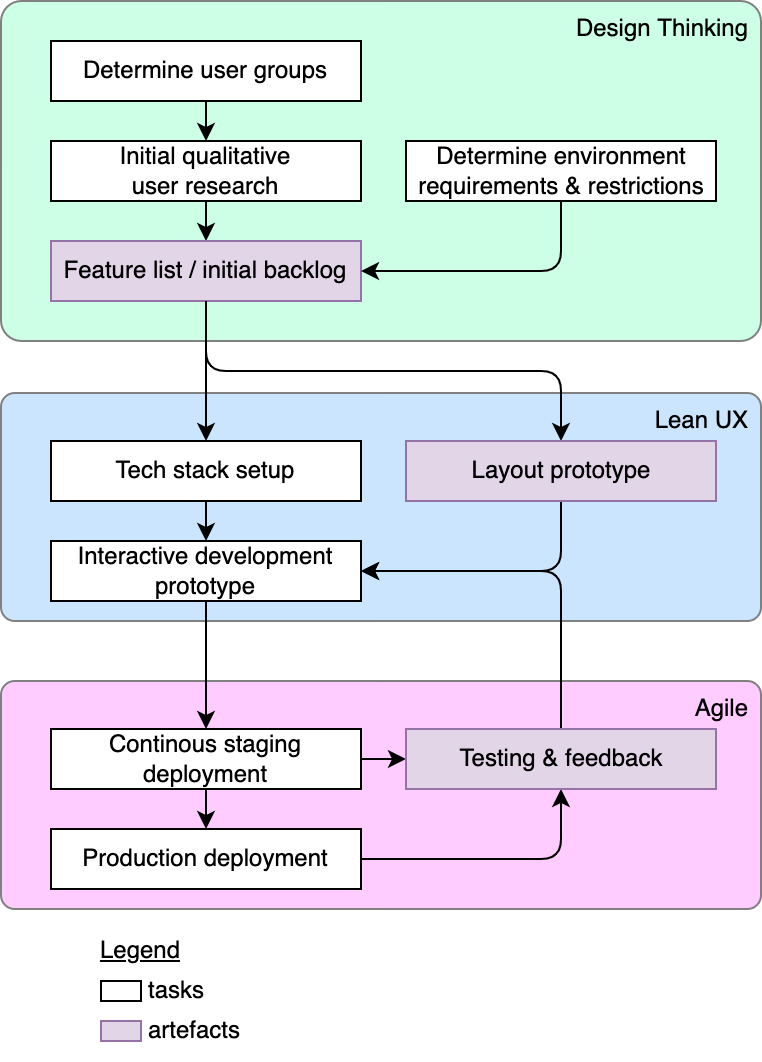
\includegraphics[width=0.8\linewidth]{pics/process.drawio.png}
  \caption{Software design process for the UI Editor.}
	\label{fig:process}
\end{figure}


% !TeX root = ../thesis_main.tex
% ---------------------------------------------------
% ----- Chapters of the template
% ----- for Bachelor-, Master thesis and class papers
% ---------------------------------------------------
%  Created by C. Müller-Birn on 2012-08-17, CC-BY-SA 3.0.
%  Freie Universität Berlin, Institute of Computer Science, Human Centered Computing. 
%
\chapter{Kapitel}
\label{chap:chapters} 

\begin{itemize}
	\item Abhängig vom Ziel der Arbeit und dem verwendeten Forschungsdesign unterscheidet sich dieser Hauptteil der Arbeit erheblich. 
	\item Eine sehr allgemeine Struktur ist die folgende:
	\begin{itemize}
		\item Hintergrund der Arbeit (Theoretische Einordnung der Arbeit) 
		 	\begin{itemize}
		 		\item Hier sollte enthalten sein, welche Anwendungen in diesem Bereich bereits existieren und warum bei diesen ein Defizit besteht. 
				\item Falls genutzt, sollten hier die entsprechenden Algorithmen erläutert werden.
				\item Es sollten die Ziele der Anwendungsentwicklung, d.h. die Anforderungen herausgearbeitet werden. Dabei sollte die bestehende Literatur geeignet integriert werden.
		 	\end{itemize}
		\item Umsetzung (Praktischer Anteil der Arbeit)
			\begin{itemize}
				\item Zunächst sollte die Softwarearchitektur und die genutzten Anwendungen, APIs etc. erläutert werden. Ebenfalls gehört dazu das Datenbankschema.
				\item Es sollten die zentralen Elemente der Software (abhängig von der Aufgabenstellung) beschrieben werden, wie implementierte Algorithmen oder das Oberflächendesign.
				\item Zentraler Quellcode sollte entsprechend aufgelistet werden:
				\lstset{language=Java,basicstyle=\footnotesize,numbers=left,showstringspaces=false,frame=single}
				\begin{lstlisting}
				public class Main {
					public static void main(String[] args) {
						System.out.println("Hello World!");
					}
				}
				\end{lstlisting} 
				%\item Klassendiagramm für Backend
				%\item Dr Quellcode zentraler Implementierungen  können als Auszug in den Anhang. Im Text kann dann darauf verwiesen werden.
			\end{itemize}
		\item Evaluation (zumeist nur für Masterarbeiten relevant)
		\begin{itemize}
			\item Jede Software muss auch getestet werden. Dieses Tests werden entweder mit einem vorgegebenen Datensatz erfolgen oder aber die Evaluation erfolgt auf Basis von Experimenten. In diesem Kapitel sollte daher entweder der genutzte Datensatz oder der experimentelle Aufbau beschrieben werden. 
		\end{itemize}
		\item Ergebnis und Diskussion
		\begin{itemize}
			\item Die Ergebnisse der Anwendung werden in diesem Kapitel vorgestellt und anschließend diskutiert. Wenn möglich sollte die Ergebnisse in Relation zu bestehenden Arbeiten in dem Bereich erörtert werden.
		\end{itemize}
	\end{itemize}  
\end{itemize}
% !TeX root = main.tex
%************************************************************************
\section{Background}
\label{sec:background}
% List relevant work by others,
% or preliminary results you have achieved with a detailed and accurate
% explanation and interpretation.
% Include relevant photographs, figures or tables to illustrate the text.
% This section should frame the research questions that your subsequent research will address. 
%************************************************************************
Please add a sentence that summarizes what this section is about and what the reader can expect.
%************************************************************************
\subsection{Context of the Project and Problem Description} 
\label{sec:context}
%************************************************************************
Explain all the surroundings that are necessary to understand the broader context of your work. If necessary, give a brief introduction to non-HCI research literature as background knowledge. It is best to include a specific scenario\footnote{Scenarios are defined as an \emph{''informal narrative description''}. \emph{''It describes human activities or tasks in a story that allows exploration and discussion of contexts, needs, and requirements. It does not necessarily describe the use of software or other technological support used to achieve a goal. Using the vocabulary and phrasing of users means that scenarios can be understood by stakeholders, and they are able to participate fully in development.''}~\cite{preeceInteractionDesignHumancomputer2015}.}. If you are designing a piece of software or graphical user interface, please specify your users and the tasks the users want to perform with your software.

%************************************************************************
\subsection{Related Work}
\label{sec:relatedwork}
%************************************************************************
This section consists of a literature review to situate your thesis in the scientific context. Which academic articles exist in your problem area, and how are they related to your work? When placing your thesis in the context of others, you need to consider other work, which uses a similar methodology or articles, who try to answer similar research questions.

\begin{table}[htb]
\small
\colorbox{bamacolor}{
\centering
\begin{tabularx}{\textwidth}{@{} r Y @{}}
	&
	\textbf{Distinction between Bachelor and Master thesis}\vspace{2mm}\\
    \textbf{B. Sc. Thesis} &
    A small literature review is mandatory, starting with the articles your supervisor provides. The related work part can also include a mini similar tool analysis if you are implementing a specific part of a software. \vspace{2mm}\\
	\textbf{M. Sc. Thesis} &
	A literature review is mandatory. If it is part of your project to choose a specific framework, then you need to conduct a short survey on existing frameworks. This also applies if you want to choose an algorithm to perform a specific task or want to design a study. \vspace{2mm}\\

\end{tabularx}
}
\end{table}

In the thesis announcement\footnote{Thesis announcements are descriptions for ''Open Theses'' on the HCC website: \url{https://www.mi.fu-berlin.de/en/inf/groups/hcc/theses/open/index.html}} already, relevant literature is provided. If this is not the case, please ask your supervisor for articles. Describing the state of the art is essential to identify the gap you would like to fill. Thus, the literature's description should clearly result in research gaps that lead to specific research questions. 


%************************************************************************
\subsection{Research Questions}
\label{subsec:question}
% Based on your overarching goal and the reviewed research, specify your research question.
%************************************************************************
In this section, you should name your research questions. Your research question should be based on the observation that prior research has a gap and some misconception. You can use words such as \emph{but} or \emph{however} to indicate this. Make sure that your emphasize the significance of your research. 
% ---------------------------------------------------
% ----- Chapters of the template
% ----- for Bachelor-, Master thesis and class papers
% ---------------------------------------------------
%  Created by C. Müller-Birn on 2012-08-17, CC-BY-SA 3.0.
%  Freie Universität Berlin, Institute of Computer Science, Human Centered Computing. 
%
% TODO remove 2 - to use auto numbering
\chapter{Related work}
\label{chap:related-work} 


TODO
% ---------------------------------------------------
% ----- Chapters of the template
% ----- for Bachelor-, Master thesis and class papers
% ---------------------------------------------------
%  Created by C. Müller-Birn on 2012-08-17, CC-BY-SA 3.0.
%  Freie Universität Berlin, Institute of Computer Science, Human Centered Computing. 
%
% TODO remove 2 - to use auto numbering
\chapter{User research and analysis}
\label{chap:research}


% Due to the limited size of the user group, the goal was not to gain <TODO> with high diversity of their demographics, but to have information saturation from fewer but more valuable insights into peolpe with diffrent workflows.

To avoid the common problem in software development where products are built based on the ideas of individual stakeholders who may not even use the product,
instead of relying on meaningful user input,
I applied various methods of user research commonly used in Human-Computer Interaction (HCI) and evaluated their effectiveness in the context described earlier.

A starting point for qualitative user research is to define the goals through the help of the SMART Criteria <TODO cite>.

For these criterias, I defined the overall goal as following:

\begin{itemize}
  \item \textbf{specfic} - improve the workflow of users modifying dynamic resources
  \item \textbf{measurable} - interviews after testing period, concerning working speed and confidence when editing resources, user tracking
  \item \textbf{assignable} - research implementation will mostly be conducted by me, with input from CTO \& product owner, connection to external users through customer service team
  \item \textbf{realistic} - new software platform which reacts quicker, prvides more safety regarding errors and is scalable and extensible in the future. Limiting factors are time (as I only have three months for the first phase, including writinh this thesis)
  \item \textbf{time-related} - the new software should have at least the same feature set and be usable by company-internal users until the end of 2022
\end{itemize}
\section{Identifying and categorizing users and user groups}

In order to effectively design and implement the UI editor, it is crucial to understand the needs and preferences of the various users and user groups who will be using the tool.
Therefore, the first step in the user research process was to identify and categorize the different users and user groups who will be using the editor.
This included both internal and external users, as well as users with different levels of experience and expertise. By understanding the characteristics and needs of each user group, we can ensure that the UI editor is tailored to their specific requirements and can be used effectively by all users.
\\
As explained earlier, because we had a preceeding, less powerfull tool to edit the resources, which was used mostly by company-internal developers and managers,
but also available to some external customers. As a first step, I collected a list of mail adresses that accessed the tool by looking at the logs, and wrote a mail to our developers who would be interested in working with me for both design phase and later as alpha and -beta testers.

Then, I derived the follwoing commomn factors from the users, most of which I personally know, which made the communication and categorization a lot easier.

\begin{itemize}
  \item \textbf{quantitative usage} There were users who relied on the tools for most of their work, while others like the external customers accessed the tool a few times a year.
  \item \textbf{common tasks} I <grob> categorized the common tasks into three groups:
    \subitem \textbf{Heavy configuration} Mostly internal devs used the tools to build new apps and websites from scratch (or derived from exisiting apps), making many modifications, from structural changes to the seperate views, menus, data sources and more, over styling and translating messages to diffrent languages.
    \subitem \textbf{Moderate configuration} Project devs and customer support people copy resources from existing apps and adapt them for new brands, which often includes changing colors and logos, adapting texts or switching authentification flows.
    \subitem \textbf{Small changes} External customers often only use the tools to exchange some ads, translations or logos, which affects a small set of files.
  \item \textbf{expertise} <kann man bei schlechter software gut erkennen, leute mit viel erfahrung checken sachen, aber ist für neue nicht intutitiv>
\end{itemize}

% ... more
\section{Qualitative user resarch}

\begin{itemize}
  \item mix interview / moderated observation
  \item experiences, outcomes, what went good and bad
\end{itemize}

\subsection{Interview}

TODO interview preparation and conduction

\subsection{Moderated observation}

TODO prep and conducting

\section{Quantitaive user research}

Not used survey / questionaire -> lay down reasons why not necessary in that situation

Tracking of user behaviours

- on site using G analytics \& (the other GDPR compliant tracking tool name??)
- using server logs to understand usage patterns

\section{Process and vizualize the outcomes of the initial user research phase}

\subsection{2x2 Opportunity Matrix}

This two-dimensional vizualization of a set of proposed features prooved helpful when prioritizing tasks with other stakeholders,
as it shows the (approximated) cost of implementation as well as the value the feature can have for users.

The matrix I used is a slightly modified adaption from \cite[p. 181]{LearnHCI:2020ys}, replaced the term ''idea originality'' on the x-axis with ''Value''.

\begin{figure}[ht]
	\centering
  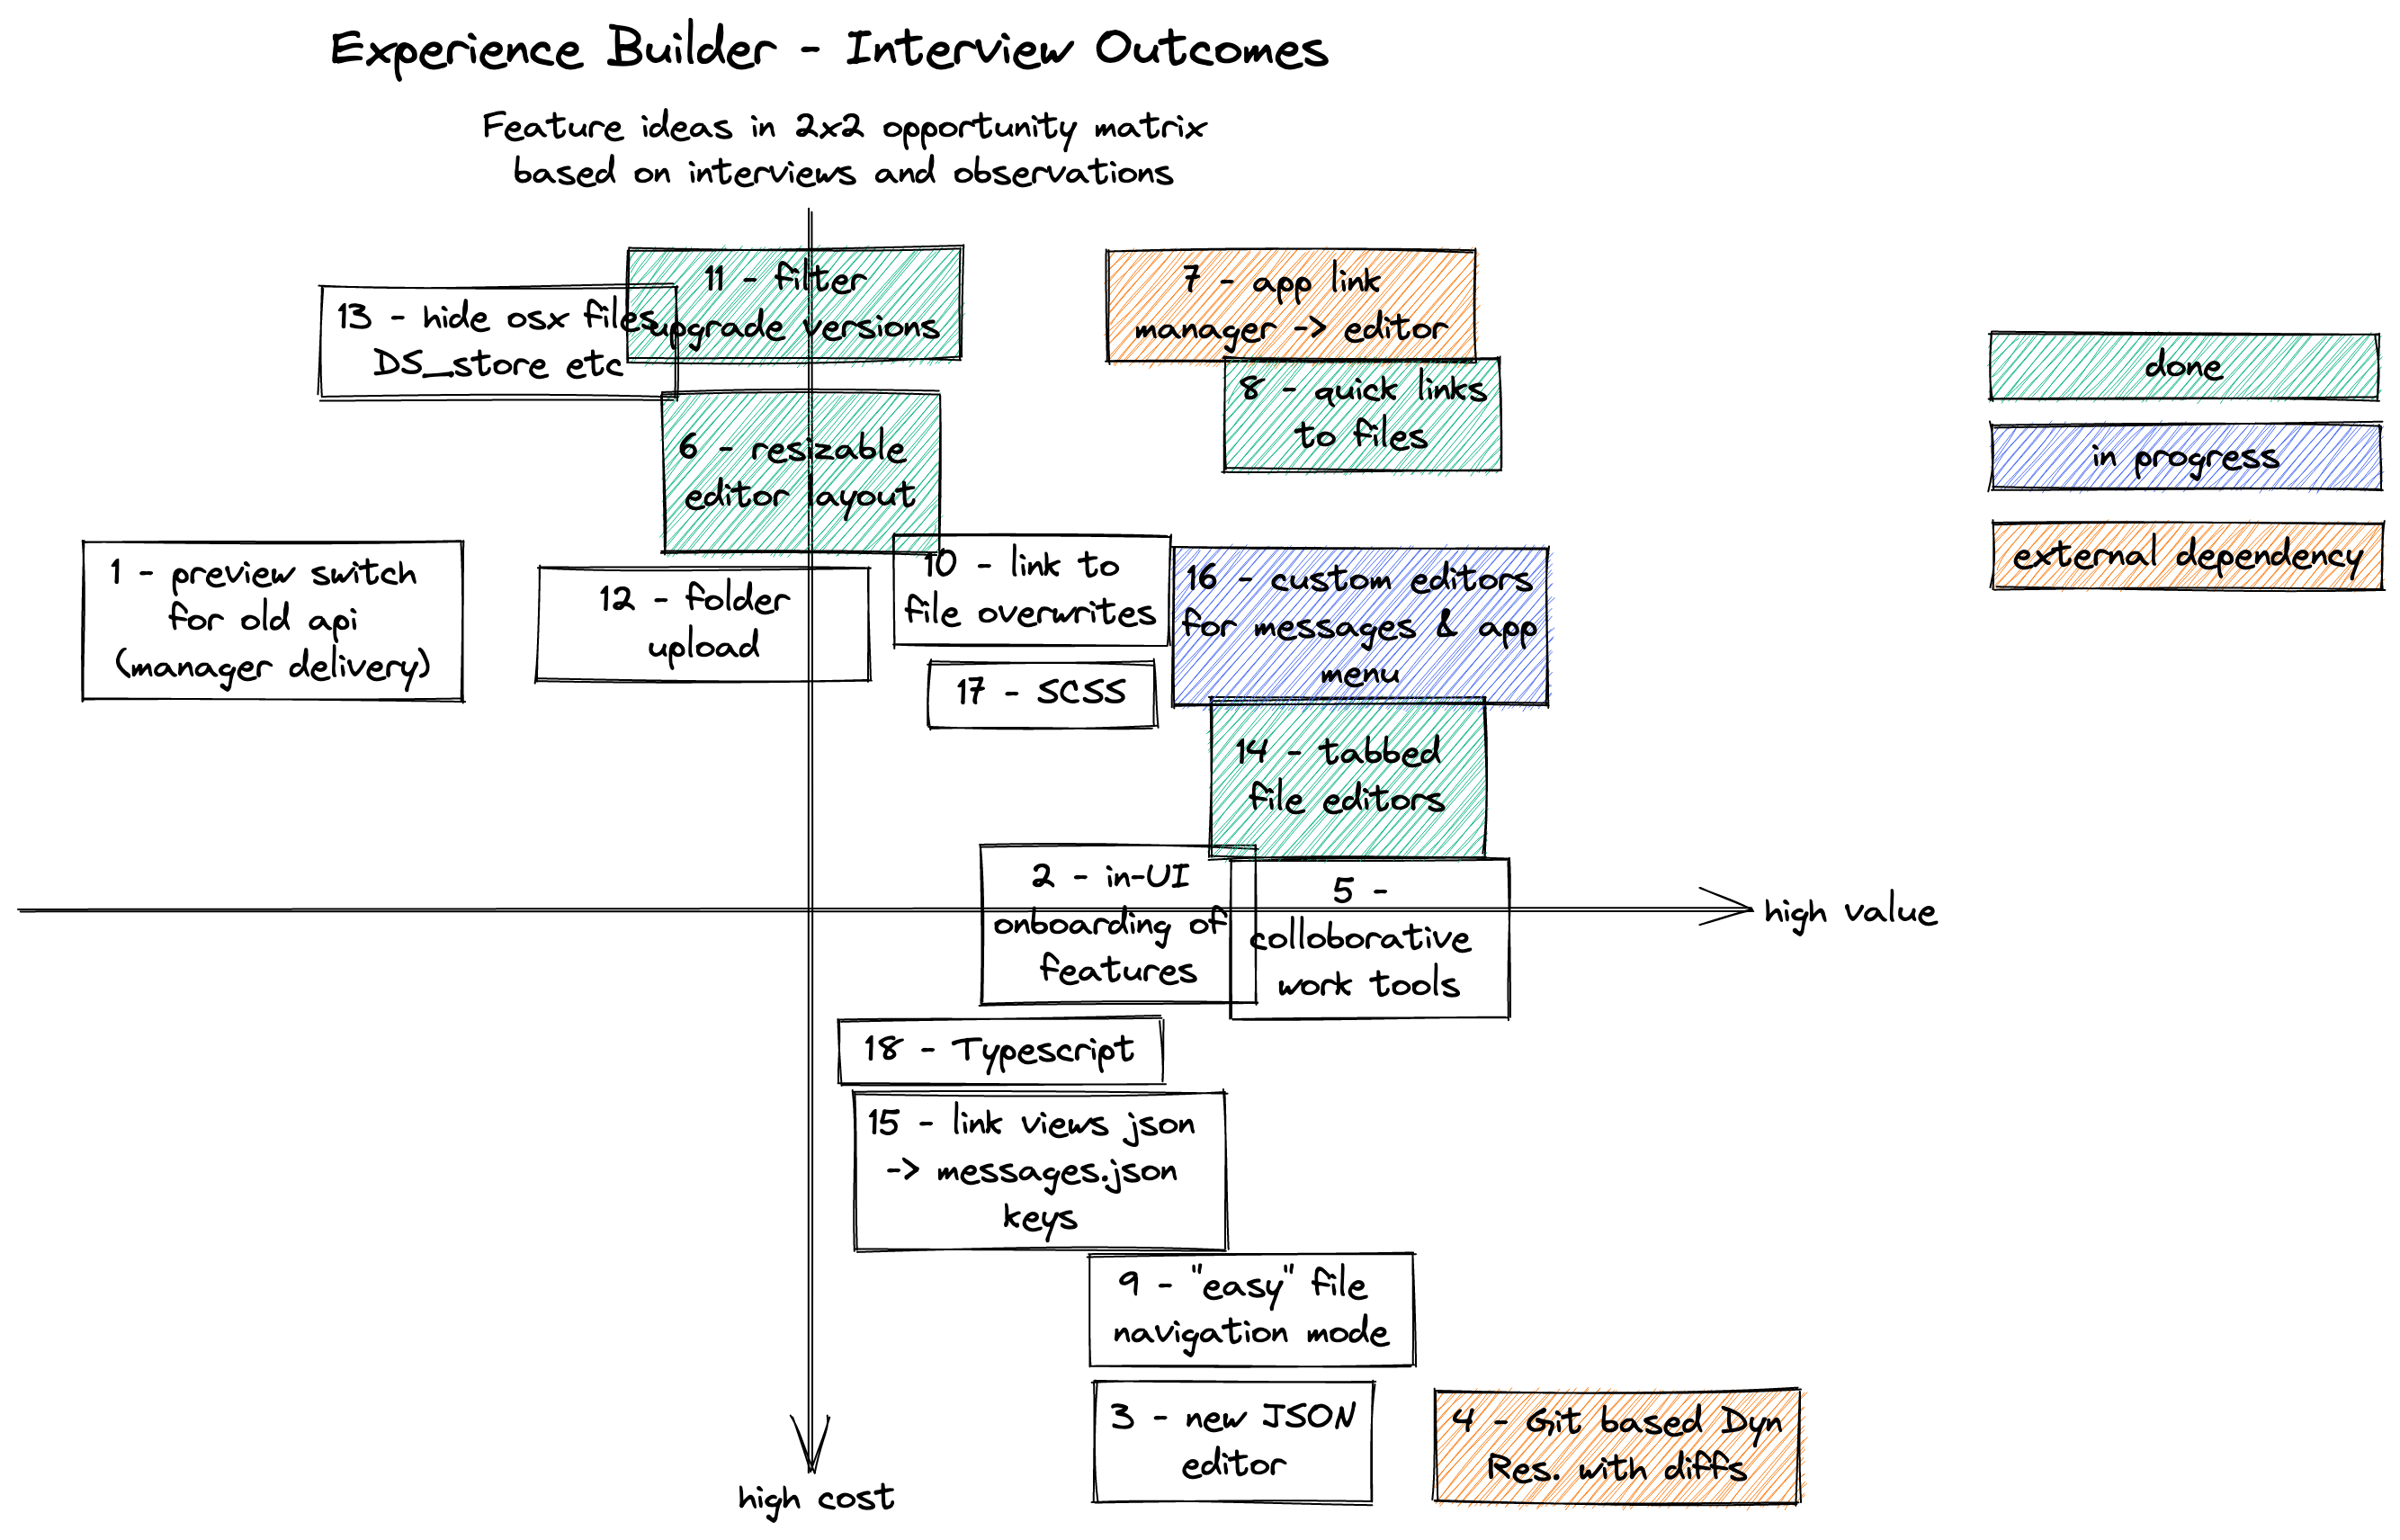
\includegraphics[width=\textwidth]{pics/feature_cost_matrix.excalidraw.png}
	\caption{2x2 Opportunity Matrix during the early phases of development}
	\label{fig:opportunitymatrix}
\end{figure}

% !TeX root = ../thesis_main.tex

% ---------------------------------------------------
% ----- Chapters of the template
% ----- for Bachelor-, Master thesis and class papers
% ---------------------------------------------------
%  Created by C. Müller-Birn on 2012-08-17, CC-BY-SA 3.0.
%  Freie Universität Berlin, Institute of Computer Science, Human Centered Computing. 
%
% TODO remove 2 - to use auto numbering
\chapter{5 - Prototyping}
\label{chap:chapters} 

After collecting the inital user feedback, I started drawing minimal digital ''paper'' prototypes using Figma to gather vizualizations of the proposed UI layouts.
Two ideas emerged from the interviews: a (file-)editor-centric layout and a preview-centric layout.
\\
The editor-centric layout is inspired by modern text editors / IDEs like VS Code (\url{https://code.visualstudio.com/}), which was mentioned as reference during the interviews multiple times.
There, the central pane is the editor for the currently open file, while in the sides additional panes for file management, preview and more can be shown.
The familarity especially to developers, who are used to IDE layouts, could help new users adopt patterns to work with the UI they use in other tools as well.
\\\\
The idea for a preview-centric layout was inspired by popular generic website builders like \url{https://wix.com} or \url{https://wordpress.com}, where the user
can see the page in an interactive mode, move, rename or place elements, and then has on the side additional panels like one with information \& options about the
currently selected one.
\\
Ultimately our choice fell to the editor centric layout, the following are some of the reasons for it over the preview-centric one:
\begin{itemize}
  \item The configuration structure of the Experience framework was not built with preview-based editing in mind. A lot of functionality is hidden inside the components and invisible for the user,
  often components only appear under specific conditions that are not easily reproducable in the editor environment. Thus, editing in a preview-centric mode could in many situations
  lead to more confusion by the editors than speed the process up.
  \item After evaluation of some avaialble libraries and examples, we concluded that building a reliable and usable preview-centric editor is more complicated, and even without the time restricition of my bachelor thesis, I proposed to not go this way,
  as it was unclear if it even could result in a viable product in reasonable time. For editor-centric UIs, many thirdparty libraries exist, that can be integrated into the UI.
  Some relevant are Monaco Editor (the VS Code Open source text editor part) for editing generic web related files like CSS and JS with automatic syntax highlighting and error detection, and an JSON Editor for work with json configs where we could provide a schema.
  \item Even though this should not be a exclusion criterion, the old tool used a editor-centric layout. Using a compeletely diffrent layout could make the switch to the new tool for users
  of the exisitng one much harder, as they have to adapt to new layout and possibly new workflow.

\end{itemize}

Figma static prototype
\\
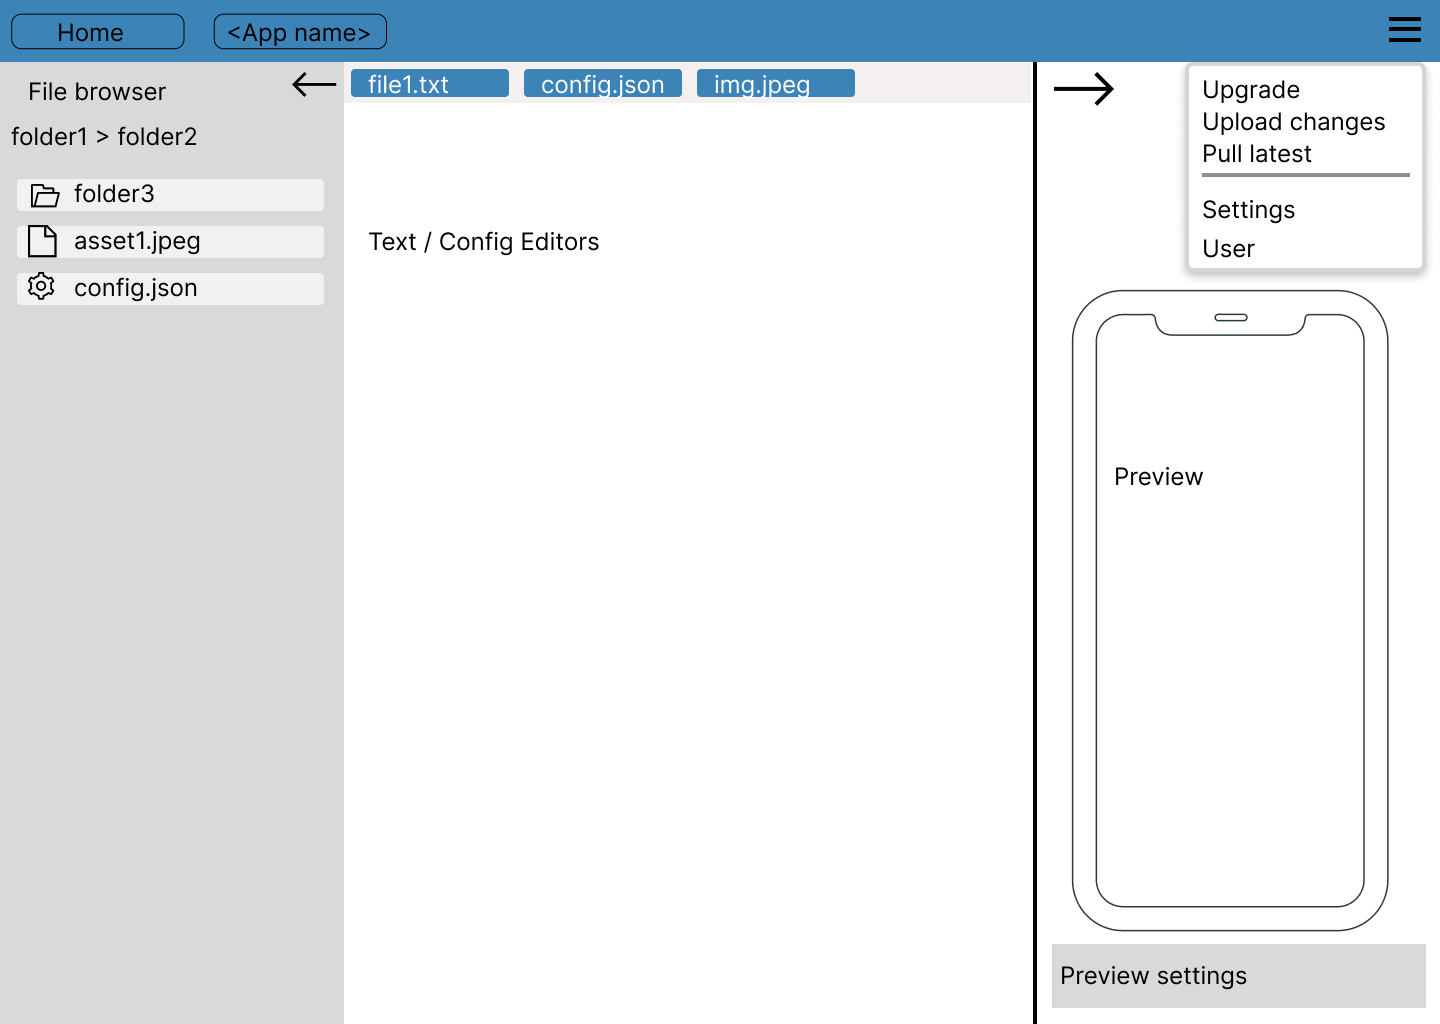
\includegraphics[width=\textwidth]{pics/figma-desktop.png}
% ---------------------------------------------------
% ----- Chapters of the template
% ----- for Bachelor-, Master thesis and class papers
% ---------------------------------------------------
%  Created by C. Müller-Birn on 2012-08-17, CC-BY-SA 3.0.
%  Freie Universität Berlin, Institute of Computer Science, Human Centered Computing. 
%
% TODO remove 2 - to use auto numbering
\chapter{6 - Implementation and deployment}
\label{chap:chapters} 


TEasfaflbaflhawlih a saf lahflahef awhj aef 
% ---------------------------------------------------
% ----- Conclusion of the template
% ----- for Bachelor-, Master thesis and class papers
% ---------------------------------------------------
%  Created by C. Müller-Birn on 2012-08-17, CC-BY-SA 3.0.
%  Freie Universität Berlin, Institute of Computer Science, Human Centered Computing. 
%
\chapter{Conclusion and outlook}
\label{chap:conclusion}      
This thesis demonstrates the challenges and opportunities of applying HCI principles and methods in a brownfield software development project through the redevelopment of a UI Editor for a digital publishing company, Sprylab.
During the process, it was shown how common user research methods can be adapted to this specific case study and how technical limits and needs of users can be combined in this context.
Agile development and Lean UX enabled iterating quickly and achieving fast deployments to a staging system.
A growing group of users at Sprylab already uses the software in production.
\\\\
The consistently positive feedback shows that the chosen methods and features derived from their outcome were the right approach to enhance the user experience while complying with constraints imposed by the ecosystem.
Also, the way users were involved during the whole process led to a high level of acceptance and interest in supporting the project.
Additionally, this thesis can help to argue for the use of HCI methods in future projects started at Sprylab as well.
I'm confident that this new software is a stable and extensible tool, especially regarding the two factors Usability and Time-on-Task.
In addition to increasing user satisfaction, it also leads to enhancing productivity and customer satisfaction.

TODO: the editor enables users to safely edit JSON configurations and change assets and styles while directly seeing these changes in a preview frame
\\\\
However, there is still room for improvements in terms of accessibility and entry hurdle for new users.
The entry hurdle is still high and a lot of background knowledge is assumed, which is partly due to the complexity of other systems in the ecosystem that were set as technical requirements from the beginning on.
Moving forward, replacing the JSON editor with a custom implementation that combines JSON Schemata and generated UI is one of the next steps, which will speed up the user's
workflow even more and allow for further improvements that are impossible with a third-party library.
\\\\
Overall, this thesis has demonstrated the importance of considering HCI principles and methods in brownfield software development projects, and the potential benefits that can be achieved when these approaches are applied in a real-world context.


%---------------------------------------------------
%----- Bibliography
%---------------------------------------------------
\phantomsection
\addcontentsline{toc}{chapter}{Literatur}
% \bibliographystyle{alpha}
\printbibliography



%---------------------------------------------------
%----- Appendix   
%---------------------------------------------------
\backmatter
% ---------------------------------------------------
% ----- Appendix of the template
% ----- for Bachelor-, Master thesis and class papers
% ---------------------------------------------------
%  Created by C. Müller-Birn on 2012-08-17, CC-BY-SA 3.0.
%  Freie Universität Berlin, Institute of Computer Science, Human Centered Computing. 
%

\chapter{Appendix}
\label{ch:Appendix}

\section{Erster Teil Appendix}
\label{app:first_appendix} 

\section{Zweiter Teil Appendix}
\label{app:second_appendix}  



\end{document}